\begin{figure}[h!]
\centering
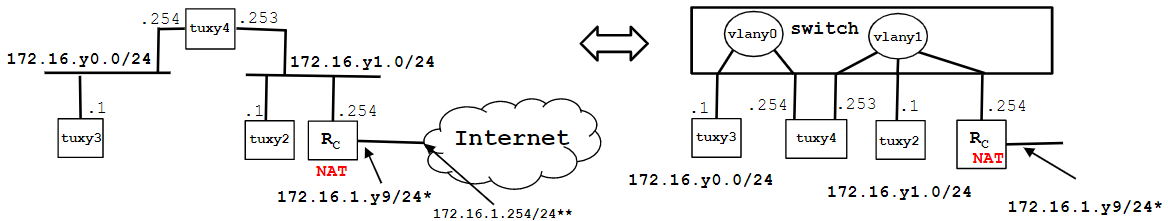
\includegraphics[scale=0.3]{imagens/Exp4.png}
\caption{Arquitetura da Quarta Experiência}
\label{fig:exp4}
\end{figure}

Esta experiência tem como objetivo estabelecer uma ligação com a rede dos laboratórios e implementar rotas num router comercial, adicionar-lhe funcionalidade NAT, e perceber qual a sua função.

Os comandos usados para esta experiência podem ser encontrados no Anexo \ref{exp4_steps}.

\subsubsection{Análise dos Logs}

O NAT (Network Address Translation), tal como o nome indica, é um mecanismo implementado em routers que substitui os endereços IP locais nos pacotes por um endereço IP público de forma a se conseguir estabelecer uma ligação para fora da rede. Sendo assim, o router que implementa o NAT torna-se responsável por encaminhar todos os pacotes para o endereço correto, dentro ou fora da rede local.

Nesta experiência, começámos por configurar a interface GE 0/0 do router \cite{cisco_config} atribuída à VLAN 21. Para a interface GE 0/1 do router, atribuiu-se o IP 172.16.1.29 para que fosse feita a ligação com a rede dos laboratórios.

Definiu-se que o tux24 serviria de router para o tux23 e o router RC para o tux22 e tux24. Adicionalmente, foram adicionadas as devidas rotas estáticas no router RC, com as instruções descritas no passo 1 do Anexo \ref{exp4_steps}.

Após estas configurações foi possível realizar o ping do tux23 a todos os outros pontos da nossa rede como a Figura \ref{fig:exp4_tux23_ping_evertything} mostra. A conexão do tux23 às interfaces dos tux's já era possível nas experiências anteriores, agora é possível também aceder às interfaces GE 0/0 e GE 0/1 do router RC, sendo isto possível uma vez que, como referido anteriormente, se adicionaram duas rotas no router RC, a default gateway com o IP 172.16.1.29 e o reencaminhamento de pacotes para a rede com IP 172.16.20.0/24 (VLAN 20 onde se encontra o tux23) através da interface eth1 do tux24 com IP 172.16.21.253.

Até ao momento a conexão do tux22 à interface eth0 do tux23 é efetuada através da rota implementada no tux22 e descrita na experiência 3. Para verificar esta implementação foi removida essa mesma rota do tux22, e executou-se o comando traceroute onde se comprova que, como não havia nenhuma rota definida até à VLAN 20, o router com o IP 172.16.21.254, definido como default gateway do tux22 ficou responsável por redirecionar os pacotes ICMP até ao destino como mostra a Figura \ref{fig:exp4_traceroute_after_remove_route} e comprovam os logs da Figura \ref{fig:exp4_tux22_ping_tux23_with_redirect}, voltando a adicionar a rota e fazendo um novo traceroute notamos que os pacotes deixam de passar pelo router e passam a seguir o "melhor caminho" via tux24, como mostra a Figura \ref{fig:exp4_traceroute_after_add_route}.

Por fim, tentamos desde o tux23 fazer ping do router do laboratório com o IP 172.16.1.254, sem sucesso uma vez que o NAT ainda não tinha sido adicionado ao router. 
Após a adição do mesmo \cite{cisco_nat}, com os comandos delineados no passo 6 do Anexo \ref{exp4_steps}, voltamos a tentar o passo anterior, com sucesso uma vez que agora, o NAT permite que os dispositivos conectados à rede local, 172.16.2x.0/24 (interface 0/0), comuniquem com a rede externa, 172.16.1.29 (interface 0/1), como comprova a Figura \ref{fig:exp4_tux23_ping_lab_router}.
